\documentclass[border=10pt]{standalone}
\usepackage{tikz,pgfplots}
\pgfplotsset{compat=1.14}
\begin{document}
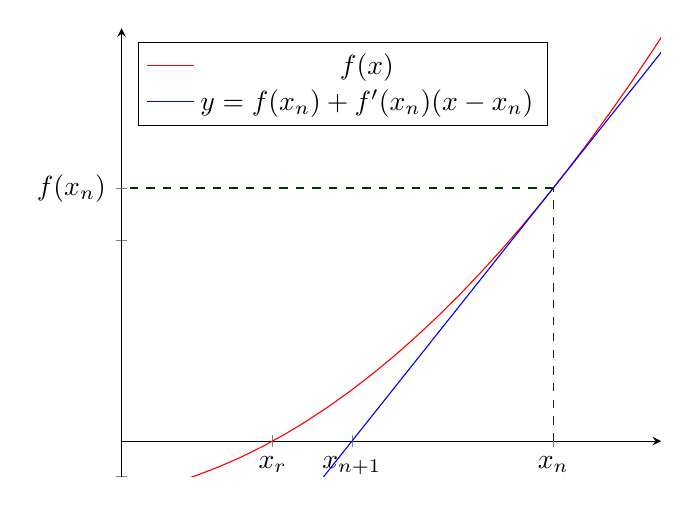
\begin{tikzpicture}
\pgfkeys{/pgf/declare function={f(\x)=(\x - 0.1)*(\x - 0.1) - 0.25;}}
    \begin{axis}[legend pos=north west,samples=200,  
    axis lines=center,
    xmin=0.25,   xmax=1.5,
    ymin=-0.15,   ymax=1.75,
    xtick={0.25,...,1.5},
    xticklabels={},
    ytick={-0.15,...,1.75},
    yticklabels={},
    extra x ticks={0.6,0.7836,1.25},
    extra x tick labels={$x_r$,$x_{n+1}$,$x_n$},
    extra y ticks={1.0724999999999998},
    extra y tick labels={$f(x_n)$}]
       \addplot [red] {f(x)};
       \addplot [blue] {2.3*(x-1.25)+1.0724999999999998};
       \addplot [green!20!black,dashed] coordinates {
        (1.25,0) (1.25,1.0724999999999998)};
        \addplot [green!20!black,dashed] coordinates {
        (0,1.0724999999999998) (1.25,1.0724999999999998)};
     \addlegendentry{$f(x)$}
     \addlegendentry{$y=f(x_n)+f'(x_n)(x-x_n)$}  
    \end{axis}
\end{tikzpicture}
\end{document}
